Using two different ancillary services and an asset management service as cases, we will illustrate the utility of the generic service modeling method, the service performance index and the service verification index. The first case study focuses on frequency containment reserve in western Denmark, the second focuses on the theoretical PowerMax DSO service, and the third focuses on the temperature management of a residential house. 

\subsection{Frequency Containment Reserve in Western Denmark}
Frequency Containment Reserve (FCR) is utilized to contain frequency excursions deviating from the nominal 50 Hz in \emph{ENTSO-E RG Continental Europe’s synchronous area} of which western Denmark (DK1) is part of. The Danish TSO, Energinet.dk, is obliged to provide a proportional share of $\pm$ 23 MW \cite{EnerginetAncillary} out of the total synchronous area need of $\pm$ 3000 MW. Energinet.dk buys these reserves at daily auctions. The service specifications are defined in \cite{EnerginetAncillary}.

The six steps outlined in Sec.~\ref{sec:SEGANmethodology} are used to model the ideal and tolerated service response. 1) The physical parameters are grid frequency (accuracy of $\pm$ 10 mHz or better), generator reserve power output, and timing of service delivery (accuracy of 1 s or better). 2) The reserve must be supplied linearly at deviations of $\pm$ 200 mHz relative to 50 Hz, with a $\pm$ 20 mHz dead-band around 50 Hz. 3) The physical size of the service depends on the reserve bid size. This work will look at a generic reserve bid. According to the discussion from Eq.~\eqref{eq:QoS}, $x_{ideal}$ cannot be equal to $\mathbf{x}_{acc}$. Therefore, a $\pm$ 1\% tolerance band of $x_{ideal}$ is assumed. 4) The first 50\% of the service must be supplied within 15 s and 100\% must be supplied within 30 s. The ideal response can be defined as a response with an instant 100\% power ramp \cite{makarov2008assessing}. 5) The ideal and tolerated response of this service provision is plotted as $x_{ideal}$, $x_{acc,min}$ and $x_{acc,max}$ in Fig.~\ref{fig:DK1PrimResSim}, which assumes that a reserve power set-point has already been established based on the values from step 2.%Fig.~\ref{fig:DK1PrimResDyn}

%\begin{figure}
%\centering
%\includegraphics[width=\columnwidth]{figures/dynresp.eps}
%\caption{DK1 Primary Reserve service provision curve. The curve shows the relationship between the activated fraction of the primary reserve bid, and the grid frequency, including the +/- 20 mHz dead-band. This should not be confused with the droop curve.}
%\label{fig:DK1PrimResDyn}
%\end{figure}

Fig. \ref{fig:DK1PrimResSim} shows a simulation of primary regulation active power ramp $x_{act}$ for the time interval $[-5,35]$ s. The service delivery performance index and non-delivery verification index are $\eta^{AS}=0.4257$ and $\epsilon^{AS}=0.1392$, calculated using Eq. \eqref{eq:etaAS} and Eq.~\eqref{eq:epsilonAS}. The TSO must determine a threshold $\epsilon_{max}$, such that the service provider is penalized or the contract is terminated if $\epsilon^{AS}>\epsilon^{AS}_{max}$. It is not the scope of this work to asses a suitable value of $\epsilon^{AS}_{max}$.%\bondynote{We are repeating ourselves a bit here}

\begin{figure}
\centering
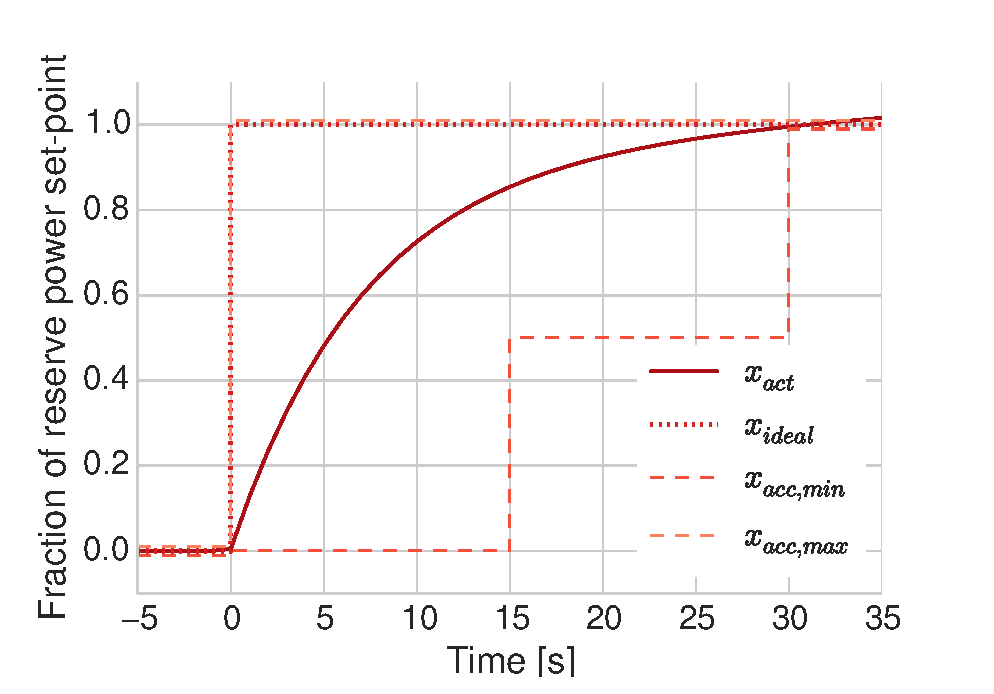
\includegraphics[width = \columnwidth]{SEGAN/primfreqresp.eps}
\caption{Simulation of a DK1 primary reserve power ramp response together with $x_{ideal}$ and $x_{acc}$ values.}
\label{fig:DK1PrimResSim}
\end{figure}

\subsection{PowerMax in a distribution system}
The \textit{PowerMax} service was first described in \cite{ding2013development} and further specified in \cite{bondy2014powermax}. It is a DSO service, where the DSO can make a tender for a load reduction $\Delta P^{DSO}$ to a max level $P_{max}^{DSO}$ in parts of the distribution system that are forecasted to experience congestions during some periods (e.g. hours 17-20 during winter months). The motivation for \textit{PowerMax} is that the service could be an economically beneficial alternative to grid reinforcements in some situations. This is both due to saved interest and depreciation on investments plus the avoided risk of over-sizing equipment in case of future energy savings or if the disappearance of a large consumer makes the reinforcement unnecessary.% The tender is announced and cleared through Flexibility Clearing House (FLECH), where flexibility aggregators can bid on the tender.%where the service is delivered by aggregator companies, which bid in flexibility from a group of units which they control. 

%Following is a mathematical definition of the \textit{PowerMax} service, as previously developed in \cite{bondy2014powermax}. 
In order to identify its service needs, it is assumed that the DSO is able to separate the total consumption forecast $\hat{P}_{tot}$ in the congested part of the distribution grid into a controllable load forecast $\hat{P}_{CL}$ and a base load forecast $\hat{P}_{BL}$:
\begin{align}
\hat{P}_{tot} &= \hat{P}_{CL} + \hat{P}_{BL} \\
\hat{P}_{CL} &= \sum_{Agg} \hat{P}_{CL,Agg}, \quad Agg \in \mathbf{A} \label{eq:CLDef}
\end{align}
where $\mathbf{A}$ is the set of all aggregators in the considered part of the grid. Only the aggregators \emph{Agg} that bid for the service tender make up $\hat{P}_{CL}$, while the rest of $\mathbf{A}$ is part of $\hat{P}_{BL}$. The aggregators must be contracted to deliver a total power reduction $\Delta P$, such that the system operational limit $\bar{P}_{sys}$ is not violated by the peak base load forecast and the peak controllable load forecast:

\begin{equation}
\hat{\bar{P}}_{BL}+\hat{\bar{P}}_{CL}-\Delta P \leq \bar{P}_{sys}. \label{eq:PSysDef}
\end{equation}

This inequality can be fulfilled by setting a peak limit $\bar{P}_{CL}$:
\begin{equation}
\bar{P}_{CL} = \hat{\bar{P}}_{CL} - \Delta P \label{eq:PBarCLDef}
\end{equation}
where $\Delta P$ and $\bar{P}_{CL}$ are the variables for the DSO service tender. In order to formulate a service tender, the magnitude of these variables must be estimated taking into account the uncertainty of the forecasts, giving the following expressions:
\begin{align}
\Delta P^{DSO} &= \sum_{Agg} \Delta \hat{P}_{CL,Agg} + \text{Risk\{}\hat{P}_{CL} + \hat{P}_{BL}\text{\}}\\
P_{max}^{DSO} &= \hat{\bar{P}}_{CL} - \Delta P_{DSO}
\end{align}
where $\Delta \hat{P}_{CL,Agg}$ is the estimated power reduction for the individual aggregator bid, $\text{Risk\{}\hat{P}_{CL} + \hat{P}_{BL}\text{\}}$ is the risk associated to the load forecast uncertainty. $Agg \in \mathbf{A_{C}}$ and $\mathbf{A_{C}} \subseteq \mathbf{A}$, i.e. $\mathbf{A_{C}}$ is the subset of aggregators that bid on the tender. After the DSO has identified a suitable $P_{max}^{DSO}$ and $\Delta P^{DSO}$ to solve the congestion issue, the DSO formulates a service tender for which aggregators can bid their corresponding $\Delta P^{Agg}$ and $P^{Agg}_{max}$. %The DSO sets a maximum price it is willing to pay for the load reduction, which is related to the alternative cost of grid reinforcements. In case the market is not cleared at or below the maximum price, the DSO can formulate a new tender, adjusting the risk value, POD (point of delivery) list or amount of power reduction. The timing of the tender process should be such that the DSO has time to conduct grid reinforcements as an alternative.

The method from Sec.~\ref{sec:SEGANmethodology} is used to model \textit{PowerMax} ideal and acceptable response. 1) The physical parameters are $P_{max}^{Agg}$, $\Delta P^{Agg}$ and months/days/hours the service shall be delivered. 2) The system does not posses a dynamic behaviour related to system parameters. 3) As an example, the service tender defines $P_{max}^{Agg} = 200$ kW and $+1\%$ allowed deviation $P_{max,acc}^{Agg}$. 4) In this example we use 120 min service provision time with allowed non-delivery in the first 15 min, and the last 5 min, of the service delivery (following the service definition in \cite{ding2013development}) and the ideal service delivery is the one that respects $P_{max}^{DSO}$. 5) Figure \ref{fig:PowerMaxSim} plots $x_{ideal}$ and $x_{acc}$. The \textit{Activation Dead-band} indicates the regions where the aggregator is not obliged to deliver the service because of the tolerances defined under step 4. 6) The service is a maximum cap service and the error is measured as in Eq.~\eqref{eq:maxmin_cap}.

An example of a load curve $P_{Agg}=x_{act}$ is presented in Fig.~\ref{fig:PowerMaxSim}. The service delivery and verification are evaluated using Eq.~\eqref{eq:etaAS} and Eq.~\eqref{eq:epsilonAS}, yielding $\eta^{AS} = 0.5074$ and $\epsilon^{AS} = 0.2701$ respectively. As with the performance assessment of the FCR in DK1, it is not within the scope of this paper to asses the value of $\epsilon^{AS}_{max}$, yet a qualified assessment can be made. %, which will lead to either penalization or termination of the contract.
To asses $\epsilon^{AS}_{max}$, the DSO must analyze the dynamics of the problem the service is helping relieve. For \textit{PowerMax}, the dynamics are governed by the heating of the overloaded equipment (e.g. transformer or cable), which deteriorates over time due to overheating. A feeder might be tolerant to short term overloads and therefore the DSO might set $\epsilon^{AS}_{max}$ higher than in the FCR case.

\begin{figure}
\centering
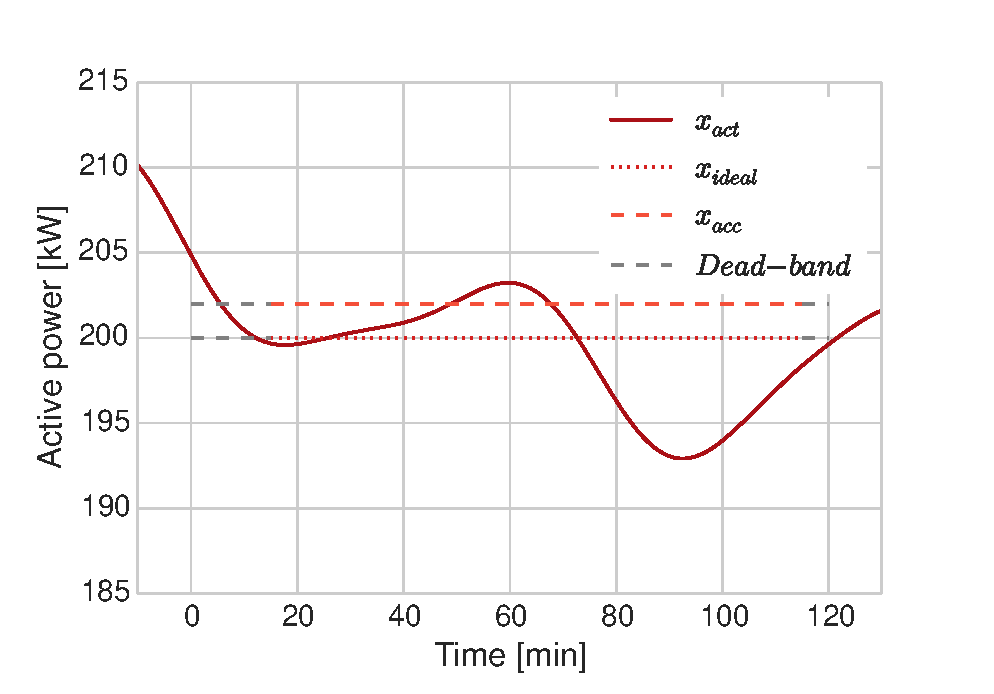
\includegraphics[width = 0.86\columnwidth]{SEGAN/powermaxsample.eps}
\vspace{-4pt}
\caption{$x_{ideal}=P_{max}^{Agg}$, $x_{acc}=P_{max,acc}^{Agg}$ for the considered \textit{PowerMax} example. The activation Dead-band is the time period, where the aggregator is allowed to non-deliver.}\label{fig:PowerMaxSim}
\end{figure}

\subsection{Temperature management of a flexible household}
Household heating is a flexible process where the thermal capacity of the building can be considered a form of energy storage. In Denmark, heat pumps are being installed with the capability of being remotely controlled by an aggregator, see e.g. \cite{insero}. It is assumed that the aggregator will help the heat pump owners to maintain a comfortable indoor temperature and utilize the electric consumption flexibility in exchange of monetary compensation.

Applying the method from Sec.~\ref{sec:SEGANmethodology} to model the service: 1) The physical parameters are the minimum and maximum of the temperature comfort bands of the household. 2) The service does not posses a dynamic behaviour related to system parameters. 3) As an example, the household owner sets a comfort band of $\mathbf{x}_{ideal} = [x_{min},x_{max}] = [20 ^{\circ}\text{C},22^{\circ}\text{C}]$ and allows for a $\pm 1 ^{\circ}\text{C}$ as acceptable error. Furthermore, the owner decides that during the night, the house can be two degrees colder. 4) In this example the ideal response is performance within the temperature bounds. 5) Fig.~\ref{fig:tempband} plots $x_{ideal}$ and $\mathbf{x}_{acc}$. 6) The service is a band service and the error is measured according to Eq.~\eqref{eq:band_error}.

The service model and the actual temperature of a simulation can be seen in Fig.~\ref{fig:tempband}, where it is clear that generally the aggregator is able to provide a reasonable service performance, with no non-delivery ( $\eta^{AMS} = 0.2707$ and $\epsilon^{AMS} = 0.0$). As described in Sec.~\ref{sec:DERs}, the aggregator may be in charge of the overall control of a cluster of units, in which case the performance should be evaluated over the whole cluster. To show this, simulations are done for 20 households and the equally-weighted average of the indices results in $\eta^{AMS} = 0.2411$ and $\epsilon^{AMS} = 0.0211$ (Fig.~\ref{fig:tempbandclustererror}).

\begin{figure}
\centering
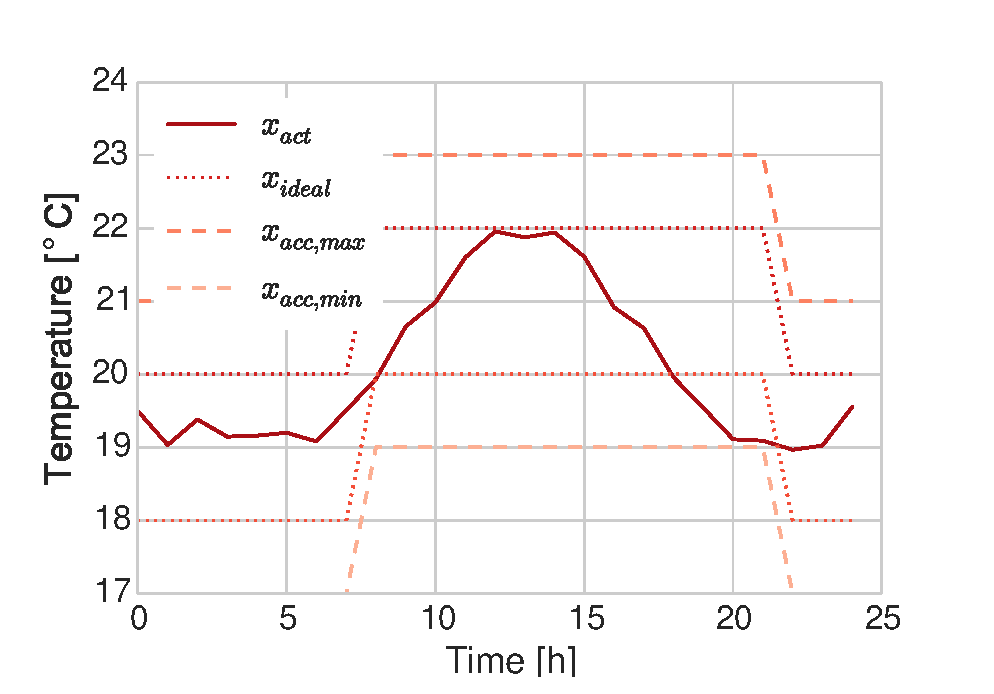
\includegraphics[width = \columnwidth]{SEGAN/tempband.eps}
\caption{Simulation of the indoor temperature of a Danish household.}
\label{fig:tempband}
\end{figure}

\begin{figure}
\centering
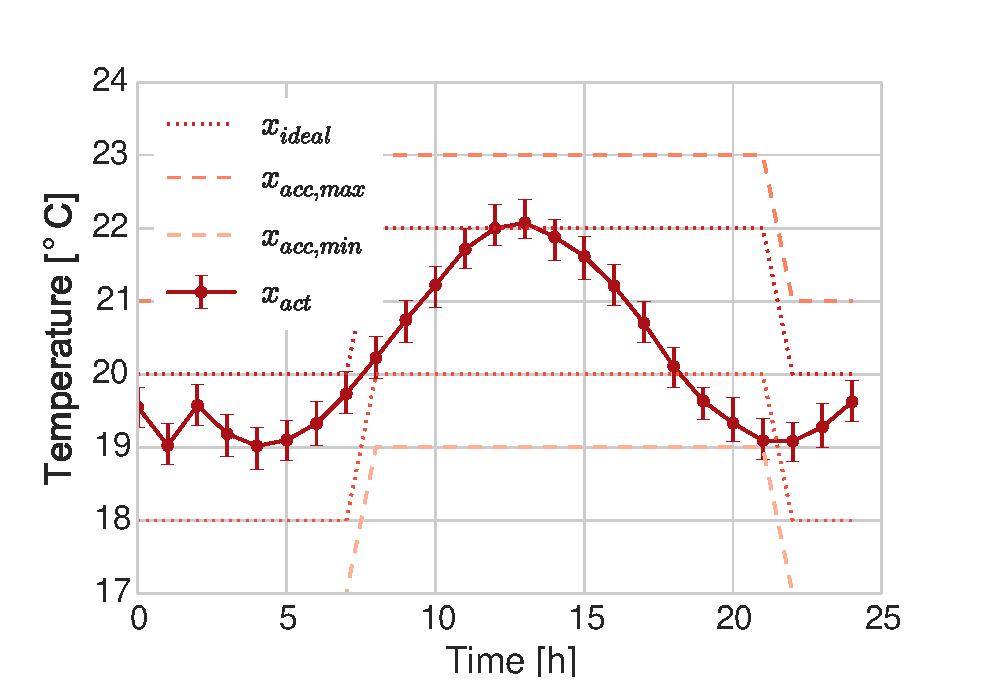
\includegraphics[width = \columnwidth]{SEGAN/tempbandclustererror.eps}
\caption{Simulation of the indoor temperature of 20 Danish households. The mean temperature is plotted, along with the minimum and maximum values of the cluster.}
\label{fig:tempbandclustererror}
\end{figure}
